\section{Neutrinos}

% █ What are neutrinos? What is neutrino astronomy?
Neutrinos are elementary particles with no electric charge and small mass. % [very] small mass…
Their low interactivity
  makes them difficult to detect,
  but is also the reason why they are valuable messenger particles for astroparticle physics:
Since they are not affected by the electromagnetic force,
% and very little by gravity,
  cosmic magnetic fields have no effect on their propagation paths \cite{neutrinos_katz}.
Neither does the interstellar medium absorb them in significant amounts.
Together with the energy of the neutrino,
  the direction of travel % / this information
  is used to determine the location and properties of the source \cite{neutrinos_katz}.


% █ Sources
%   - Nuclear reactors
%   - Solar
%   - AGNs
%   - Supernovae
%   - Atmospheric neutrinos
Neutrinos have various astronomical sources,
% \todo{We are not sure about these!}
including
  …. % TODO
  % supernovae,
  % pulsars, % Oxford comma
  % and active galactic nuclei.
Neutrinos are also produced in
  the Sun
  and in the Earth's atmosphere
  as well as in nuclear reactors.
They cover a vast range of energies, from \si{\micro\electronvolt} up to \si{\peta\electronvolt},
  depending on the source. \citationneeded{}
\autoref{fig:neutrinos:flux_spectrum} shows the flux spectrum of neutrinos from different sources.

\icecube{}
  (without \emph{DeepCore} and \emph{IceTop})
is sensitive to
  the energy range from \si{\tera\electronvolt} to \si{\peta\electronvolt} \cite{icecube_aartsen}
  and therefore primarily to atmospheric and AGN neutrinos.
%
Atmospheric neutrinos are produced by the interaction of cosmic rays with the Earth's atmosphere.
Cosmic rays are high-energy particles
  % mostly protons
  [that originate from supernovae and other sources in the galaxy].


% One can see
%   the abundance of medium-energy neutrinos from the Sun,
%     for example,
%   as well as the scarcity of (hypothesized?) high-energy neutrinos from AGN (active galactic nuclei),
%     which \icecube{} is sensitive to.

\begin{figure}
  \centering
  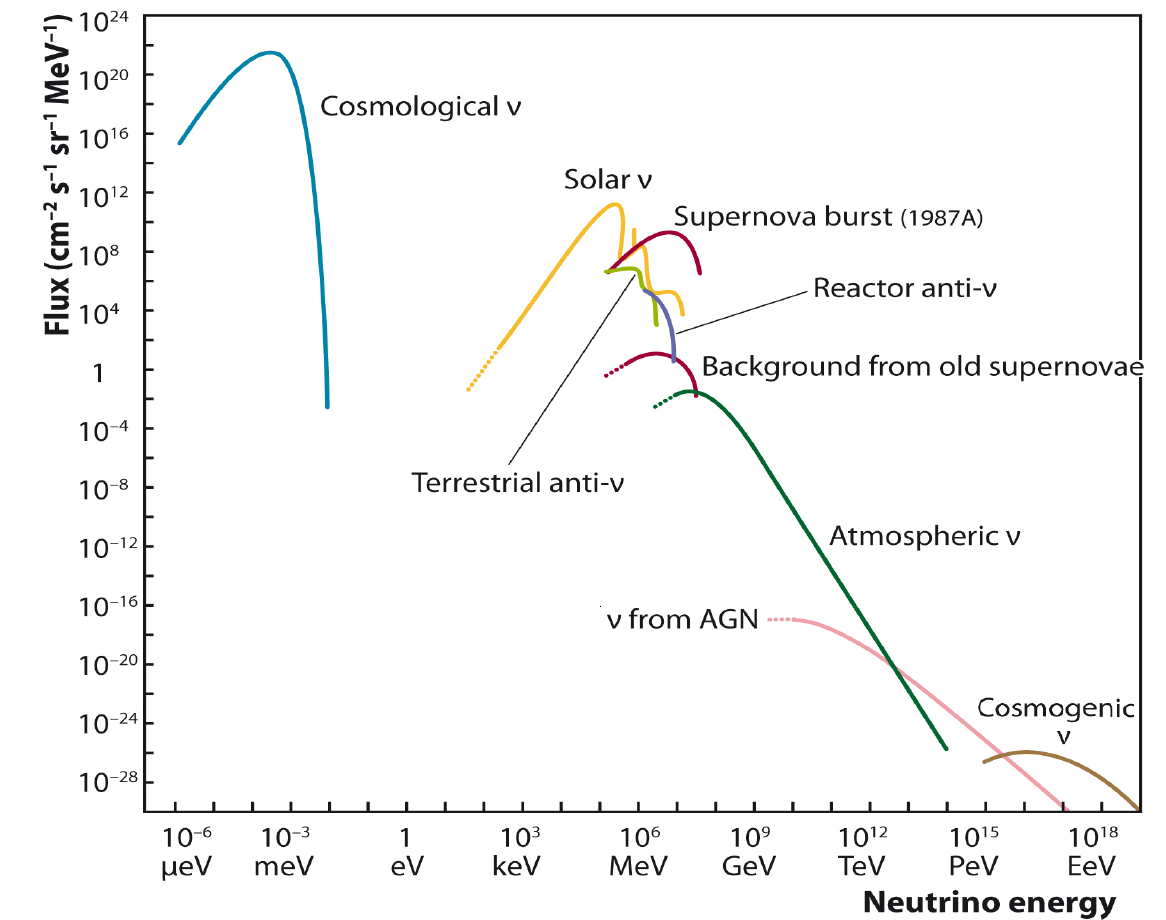
\includegraphics[width=0.75\textwidth]{content/plots/halftime/neutrinos-energy.png}
  \caption{
    Neutrino flux and corresponding source classes as a function of their energy.
    \cite{spiering2012} % We use a colorized adaption; no better source found.
  }
  \label{fig:neutrinos:flux_spectrum}
\end{figure}


% █ Neutrino oscillations
While current models of astrophysical neutrino sources predict a flavor ratio of
  $\phi(\nu_e) : \phi(\nu_\mu) : \phi(\nu_\tau) = 1 : 2 : 0$
    (assuming charged pions decays are the dominant mechanism for neutrino production),
the observed ratio on Earth is
  $1 : 1 : 1$ \cite{neutrinos_beacom}.
This discrepancy is explained by neutrino oscillations \cite{neutrinos_beacom},
  which are a consequence of the fact that neutrinos have mass.
Albeit being very small
  (the current lowest upper limit on the Majorana mass being \qtyrange{0.06}{0.161}{\electronvolt} \cite{neutrinos_gando}),
  it allows for oscillations between the different flavors,
    given the large distances that cosmic neutrinos travel.
